\section{Active Learning Approaches}
\label{sec:approach}
We first give an overview of the AL framework and then present some 
traditional and commonly used sampling strategies before presenting 
two new techniques we developed in this work. 

\subsection{Active Learning Framework}

Given a dataset $ \mathcal{Z}$, which contains $D$-dimensional feature vector as well as few labels $y_i \in \{0,1,...,K\}$ , 
$\mathcal{Z}$ will be divided into unlabeled $\mathcal{U}_t$ and 
labeled $\mathcal{L}_t$ at time step $t$. 
% \KZ{I think the above wording is confusing. If Z already contains x and y, how come $U_t$ is
% called unlabeled?}
% \KZ{Why talk about fastText here?  
% fastText works as a probabilistic classifier $f$ which can generate hidden layer feature 
% $h(x)$ and map features to probability vector.} 
The AL sampling strategy defines a utility function $\mathcal{V}(x)$ and selects and queries 
the point with the highest $\mathcal{V}(x)$ at $t$, i.e., $x^*=\argmax_{x_i\in\mathcal{U}_t}\mathcal{V}(x_i)$.
We then remove $x^*$ from $\mathcal{U}_t$ and 
add it to $\mathcal{L}_t$ by labeling $x^*$, train the classifier again and add $t$ by one. In order to save time and computing resource, we choose batch AL, i.e., selecting 
the top $\mathcal{B}$ points 
instead of one best point every iteration.


\subsection{Traditional Sampling Strategies}

\textbf{Random sampling (R)} is the simplest sampling strategy , to randomly select from unlabeled dataset 
$\mathcal{U}_t$. Since the true data class distribution remains unknown, 
we assume it being the uniform distribution with replacement and generate random samples.

\noindent
\textbf{Uncertainty sampling (US)} selects data points that the current classifier $f$ 
is most uncertain about. A lot of uncertainty definitions can be used and 
in our experiments, we select entropy, the most prevalent one: 
$\mathcal{V}(x_i) =  \mathcal{H}(x_i)$
    where $\mathcal{H}$ can be calculated as $ \mathcal{H}(x_i) = -\sum_{j=1}^K p(\hat{y}_i=j|x_i) log  p(\hat{y}_i=j|x_i)$ and $p(\hat{y}_i=j|x_i)$ is the output of classifier indicating the probability of label $j$ given $x_i$ at time step $t$.
    
\noindent
\textbf{Least confidence sampling (LC)} selects the instance having the least confidence in its probability vector:
%\begin{equation}
$\mathcal{V}(x_i) = - \argmax_{k \in \{0,1,..,K\}}(p(\hat{y}_i=k|x_i))$.
%\end{equation}
    
\noindent
\textbf{K-center greedy sampling (KG)}~\cite{sener2017geometric} selects the instance dependent on the classifier prediction in order to find center point instead of outlier points.
%\begin{equation}
    $\mathcal{V}(x_i) = \min_{x_j \in \mathcal{L}_t}\delta(x_i,x_j)$
%\end{equation}
where $\delta(x_i,x_j)$ denotes the distance between point $x_i$ and $x_j$. In our case, we use Euclidean distance.
    
\noindent
\textbf{Weighted uncertainty (WU)}~\cite{zhao2017deep} is an adaptive approach specially designed for RNN based on traditional uncertainty sampling, which combines representative with uncertainty. In other words, this method to some extent ease the effect of outlier. The sampling formula is shown as follows:
    %\begin{equation}
    $\mathcal{V}(x_i) = \mathcal{H}(x_i) \mathcal{S}(p(\hat{y}_i|x_i))$
    %\end{equation}
    where $\mathcal{H}(x_i)$ is calculated as in US, while $\mathcal{S}$ is calculated according to the following procedure. 
    In hidden feature space, we calculate the centroid of each label by averaging the feature vector of all samples from $\mathcal{U}_t$ belonging to the label according to classifier prediction. Then, for a certain data point, we calculate the cosine similarity between the centroid of its predicted label. This similarity score is treated as representativeness $\mathcal{S}$.  For convenience of notation, we assume $\hat{y_i} = k$ and denote the set of points whose predicted label is $k$ as $\mathcal{U}_k$. 
    $\mathcal{S}(\hat{y_i} = k|x_i) = \frac{h(x_i) \cdot C_k}{||h(x_i)|| \cdot ||C_k||}$ where $h(x_j)$ is hidden feature of $x_j$ and 
    $C_k = \frac{1}{|\mathcal{U}_k|} \sum_{x_j \in \mathcal{U}_k} h(x_j)$.

%  The general algorithm is shown as follows: \KZ{If this is the original algorithm
% presented in the cited paper, then we can omit it.}
%  \begin{algorithm}
% \caption{Weighted Uncertainty}
% \label{alg:WU}
% \begin{algorithmic}
% \STATE {Randomly select a small dataset $L_t \subset Z$ and label it. The remaininng  data $U_t = Z \setminus L_t$ is the unlabeled pool with $t = 0$.} 
% \REPEAT 
% \STATE Calculate the entropy score $\mathcal{H}(x)$.
% \STATE{Calculate the center of each predicted class $C_k$.}
% \STATE Calculate the similarity score $\mathcal{S}(\hat{y_i} = k|x_i)$.
% \STATE Sort $V(X_i) = \mathcal{H}(x_i) \mathcal{S}(p(\hat{y}_i|x_i)) $ and select the top $B$ data points.
% \STATE{Label the batch data selected and train $f_{t+1}$ using $L_{t+1} = L_t \cup B$.}
% \UNTIL{Model meet the accuracy qualification}
% \end{algorithmic}
% \end{algorithm}


We propose to model the representativeness of a sample
point in a different way (see \secref{sec:classradius}). To solve oversampling problem in many-class classification task, we utilize frequency of predicted class in the label pool to smooth the scoring function $\mathcal{V}(x)$ (see \secref{sec:classfreq}).

\begin{figure}[th]
\centering
\scriptsize
\small
\setlength{\abovecaptionskip}{0pt}
\setlength{\belowcaptionskip}{0pt}
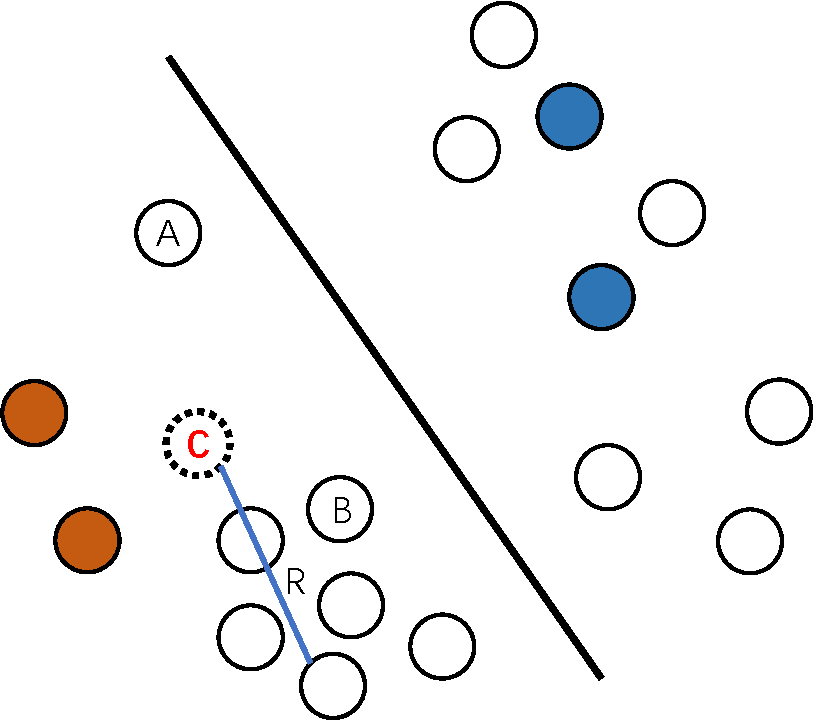
\includegraphics[scale=0.3]{figs/radius.pdf}
\caption{Geometric meaning of radius. Points on the left and points on the right
belong to different classes. A, B are data points and C is the hypothesis center. 
R denotes the maximum Euclidean distance between C and points on the left.}
\label{fig:radius}
\end{figure}

\subsection{Uncertainty with Class Radius (RU)}
\label{sec:classradius}
We want to utilize $\mathcal{X}$ to improve the sampling quality. 
WU also takes into account $\mathcal{X}$ but depends too much on the 
intermediate classifier output. It calculates the distance
between unlabeled data point and hypothesis center. 
However, the classifier trained at the early stage
is inaccurate and the hidden vectors are not reliable. 
So the distance will be quite different from the true distance. 
In order to alleviate the distortion by such immature classifiers, we relax the condition of evaluating the representative of each point and define class radius score $\mathcal{R}(\hat{y_i}=k|x_i)$ to measure the value of each class: 
%Like weighted uncertainty, we combine the uncertainty along with radius score.
    
\begin{equation}
\mathcal{V}(x_i) = \frac{\mathcal{H}(x_i)} {\mathcal{R}(\hat{y_i}=k|x_i)}
\end{equation}
    
The radius score $\mathcal{R}(\hat{y_i}=k|x_i)$ can be calculated as follows. First, we obtain the hypothesis center point of each class by averaging the feature vector of all data points classified into this class. We define radius as the maximum Euclidean distance between center point and points belonging to this class. Figure \ref{fig:radius} shows the geometric meaning of radius.
\begin{tabularx}{\textwidth}{@{}XXX@{}}
    \footnotesize
    \begin{equation}
        C_k = \frac{1}{|\mathcal{U}_k|} \sum_{x_j \in \mathcal{U}_k} h(x_j)
    \label{eqn:1}
    \end{equation} &
    \begin{equation}
        \mathcal{R}(\hat{y_i}=k|x_i) = \max_{x_j \in \mathcal{U}_k} \sqrt{||x_j - C_k||_2} 
    \label{eqn:2}
    \end{equation}
\end{tabularx}


    
Instead of querying representative and informative points, we prefer to choose points which belong to the class with the smallest radius. 
In other words, we hope to give the classifier the most margin at initial state by selecting a point whose class radius is small. Moreover, since many points may share the same radius score, we combine it with uncertainty score such that we can select point that is uncertain but it is easy to represent the whole class due to the small class radius.
    
WU relies too much on the classifier, and any small noises will change the center and thus amplifies the change on the similarity scores on some points, while our proposed approach is more robust since slight changes of the center position in most cases will not influence on a class with large radius.
    
\subsection{Adjustment on Class Frequency}
\label{sec:classfreq}
The increase of number of classes deprecates the performance of
existing sampling strategies. Because most of the strategies are designed 
for binary classification problems, often causing over-sampling of 
one single class. However, for many-class classification tasks, 
over-sampling of certain classes will lead to dramatic decrease in performance. 
Take an extreme situation as example, for a 50-class classification tasks, 
if we only query one class and obtains 100\% accuracy in this class, 
the overall macro F1 is still disappointingly 0.02. 
In order to solve this problem, we add a frequency adjustment feature 
$\mathcal{F}$ which can be combined with most probability-based 
sampling strategies including all the methods we introduced earlier. 
Moreover, in order to broadcast the effect of frequency feature, 
we scale the $V(x_i)$ into [0,1] by using a MinMax algorithm and the frequency score $\mathcal{F}$ can be calculated according to the rank of the labeled set, where $\mathcal{L}_k$ is the labeled set of label $k$. We sort the labels in ascending order and the labels of the same size have the same rank. For example, if label $i$ and label $j$ have 0 sample in labeled set, their frequency score is 1. If label $k$ have 1 sample, its frequency score is 2. The total formula is shown in Equation \ref{eqn:5}.

\begin{equation}
\scriptsize
\small
\mathcal{V}_s(x_i) = \frac{V(x_i)-\min_{x_j\in U}V(x_j)}{\max_{x_j\in U}V(x_j) - \min_{x_j\in U}V(x_j)}. 
\label{eqn:3}
\end{equation}

\begin{tabularx}{\textwidth}{@{}XXX@{}}%{@{}XXX@{}XXX@{}}
    \scriptsize
    %\begin{equation}
	%\mathcal{V}_s(x_i) = \frac{V(x_i)-\min_{x_j\in U}V(x_j)}{\max_{x_j\in U}V(x_j) - \min_{x_j\in U}V(x_j)}. 
	%\label{eqn:3}
    %\end{equation} &
    \small
    \begin{equation}
    \mathcal{F}(\hat{y_i} = k|x_i) = Rank(\mathcal{L}_k).  
    \label{eqn:4} 
    \end{equation}&
    \small
    \begin{equation}
    V'(x_i) = \mathcal{V}_s(x_i)F(\hat{y_i} = k|x_i).
     \label{eqn:5} 
    \end{equation}
\end{tabularx}



To show it clearly, we take the algorithm radius uncertainty with adjustment on frequency as an example in Algorithm \ref{alg:RUF}.
\begin{algorithm}
	\scriptsize
	\small
\caption{Radius Uncertainty with Frequency}
\label{alg:RUF}
\begin{algorithmic}
\STATE {Randomly select a small dataset $L_t \subset Z$ and label it. The remaining  data $U_t = Z \setminus L_t$ is the unlabeled pool with $t = 0$.} 
\REPEAT 
\STATE Calculate the entropy score $\mathcal{H}(x)$ and the center of each predicted class $C_k$.
\STATE Assign $R_k$ as the largest distance of $x_i$ (whose $\hat{y}_i = k$) to the center $C_k$.
\STATE Calculate $\mathcal{F}(\hat{y_i} = k|x_i) = Rank(\mathcal{L}_k)$ and $V(x_i) = \frac{\mathcal{H}(x_i)}{\mathcal{R}(\hat{y_i}=k|x_i)}$.
\STATE  Calculate $V_s(x_i) = \frac{V(x_i)-\min_{x_j\in U}V(x_j)}{\max_{x_j\in U}V(x_j)-\min_{x_j\in U}V(x_j)}$ .
\STATE Sort $V’(x_i) = \mathcal{F}(x_i) V_s(x_i), x_i \in U_t$ and select the top $B$ data points.
\STATE{Label the batch data selected and train $f_{t+1}$ using $L_{t+1} = L_t \cup B$.}
\UNTIL{Model meet the accuracy qualification.}
\end{algorithmic}
\end{algorithm}
\vspace{-0.3cm}